\section{Rancangan Sistem}

Sistem yang dirancang merupakan sistem \textit{checkout} otomatis untuk mengenali dan menghitung lauk Nasi Padang menggunakan YOLO11-seg. Sistem dirancang sebagai \textit{proof-of-concept} mekanisme \textit{self-service} bagi pelanggan \textit{dine-in}, di mana pelanggan dapat mengambil lauk secara mandiri kemudian meletakkan piring pada area pengambilan citra untuk dilakukan proses \textit{checkout}.

Pada sistem ini, kamera ditempatkan pada posisi tetap di atas area pengambilan citra untuk memperoleh citra piring yang berisi lauk pilihan pelanggan. Citra tersebut kemudian diproses menggunakan model YOLO11-seg yang telah dilatih untuk mengenali sembilan kelas, yaitu nasi, rendang, ayam goreng, perkedel, sayur nangka, daun singkong, telur dadar, telur kari, dan sambal. Model menghasilkan prediksi kelas dan \textit{segmentation mask} untuk setiap instans lauk yang dikenali.

Sebelum dapat digunakan pada proses \textit{checkout}, model YOLO11-seg terlebih dahulu melalui tahap pelatihan. Tahap tersebut dimulai dari pengumpulan citra Nasi Padang, anotasi setiap instans lauk, pembagian dataset, serta augmentasi pada data pelatihan. Dataset yang telah disiapkan kemudian digunakan untuk melatih YOLO11-seg sehingga model dapat mempelajari karakteristik visual dari masing-masing kelas lauk.

Setelah proses pelatihan selesai, model yang diperoleh digunakan pada tahap inferensi. Pada tahap ini, setiap hasil prediksi diperlakukan sebagai satu instans lauk dan dikelompokkan berdasarkan kelasnya. Jumlah instans pada setiap kelas kemudian digunakan oleh program kalkulasi harga. Program mencocokkan kelas lauk dengan harga tetap yang telah ditentukan dan menghitung total harga berdasarkan jumlah instans yang dikenali.

Perancangan sistem dilakukan melalui beberapa tahap yang mencakup perencanaan sistem, analisis kebutuhan sistem, dan perancangan alur sistem secara lebih rinci. Perencanaan sistem membahas tahapan yang diperlukan mulai dari persiapan dataset hingga model dapat digunakan pada proses \textit{checkout}. Analisis sistem membahas kebutuhan yang diperlukan dalam pengembangan sistem, sedangkan perancangan sistem membahas alur pelatihan, inferensi, penghitungan instans, dan kalkulasi harga.

\subsection{Perencanaan Sistem}

Perencanaan sistem \textit{checkout} otomatis Nasi Padang dilakukan melalui beberapa tahap yang dimulai dari persiapan data hingga model dapat digunakan dalam proses \textit{checkout}. Tahap awal dilakukan dengan mengumpulkan citra Nasi Padang yang memuat objek dari kelas yang akan dikenali. Citra yang telah dikumpulkan kemudian diperiksa dan dipilih agar dapat digunakan sebagai dataset dalam penelitian.

Setiap citra yang digunakan pada proses pelatihan selanjutnya diberikan anotasi untuk menunjukkan kelas dan area dari setiap instans lauk. Anotasi dibuat dalam bentuk \textit{segmentation mask} sehingga setiap objek pada citra memiliki informasi kelas dan batas objek yang digunakan sebagai \textit{ground truth} pada proses pelatihan YOLO11-seg.

Dataset yang telah dianotasi kemudian dibagi menjadi data pelatihan, validasi, dan pengujian. Pembagian dilakukan sebelum proses augmentasi agar citra hasil augmentasi tidak tersebar pada bagian dataset yang berbeda. Augmentasi hanya diterapkan pada data pelatihan untuk menambah variasi citra yang digunakan selama proses pembelajaran model \cite{yang2022augmentation,tampu2022}.

Data pelatihan selanjutnya digunakan untuk melatih YOLO11-seg. Pada proses pelatihan, model menerima citra beserta \textit{ground truth} dan menghasilkan prediksi lokasi objek, kelas, serta \textit{segmentation mask}. Hasil prediksi dibandingkan dengan \textit{ground truth} untuk memperoleh nilai \textit{loss}, kemudian bobot model diperbarui melalui proses \textit{backpropagation}. Proses tersebut dilakukan secara berulang hingga diperoleh model akhir yang digunakan pada tahap inferensi.

Pada tahap inferensi, citra piring yang diperoleh dari kamera diberikan kepada model yang telah dilatih. Model menghasilkan sejumlah instans objek yang masing-masing memiliki informasi kelas dan \textit{segmentation mask}. Setiap instans yang dikenali kemudian dihitung berdasarkan kelasnya sehingga diperoleh jumlah lauk dari masing-masing kelas.

Hasil penghitungan tersebut selanjutnya diteruskan ke program kalkulasi harga. Program mencocokkan setiap kelas lauk dengan harga tetap yang telah ditentukan, kemudian menghitung subtotal berdasarkan jumlah instans pada kelas tersebut. Seluruh subtotal dijumlahkan untuk menghasilkan total harga yang harus dibayarkan pada proses \textit{checkout}.

Tahap persiapan dataset yang digunakan dalam perencanaan sistem dijelaskan lebih lanjut pada subbagian berikut.

\subsubsection{Pengumpulan Data}

Tahap pengumpulan data dilakukan untuk memperoleh citra Nasi Padang yang akan digunakan dalam proses pelatihan dan pengujian model YOLO11-seg. Data yang dikumpulkan berupa citra piring Nasi Padang yang memuat satu atau lebih lauk dari kelas yang digunakan dalam penelitian.

Pengumpulan citra dilakukan melalui dua sumber, yaitu pengambilan citra secara langsung dan pengumpulan citra dari internet. Pengambilan citra secara langsung dilakukan untuk memperoleh citra yang sesuai dengan kondisi penggunaan sistem, sedangkan citra dari internet digunakan untuk menambah variasi tampilan lauk, seperti bentuk, penyajian, posisi objek, dan kondisi pencahayaan.

Citra yang dikumpulkan kemudian melalui proses seleksi sebelum digunakan sebagai dataset. Citra yang tidak menampilkan objek dengan cukup jelas, memiliki kualitas yang terlalu rendah, merupakan duplikat, atau memiliki elemen visual yang menutupi sebagian besar objek tidak digunakan. Seleksi tersebut dilakukan agar citra yang digunakan tetap memberikan informasi visual yang memadai untuk proses anotasi dan pelatihan model.

Dataset difokuskan pada sembilan kelas yang digunakan dalam sistem, yaitu nasi, rendang, ayam goreng, perkedel, sayur nangka, daun singkong, telur dadar, telur kari, dan sambal. Satu citra dapat mengandung lebih dari satu kelas maupun lebih dari satu instans dari kelas yang sama. Kondisi tersebut diperlukan karena pada penggunaan sistem, satu piring dapat berisi beberapa jenis lauk secara bersamaan.

Selain citra dengan objek yang terlihat secara terpisah, dataset juga dapat memuat citra dengan kondisi objek saling bersentuhan atau mengalami oklusi. Kondisi oklusi tidak diasumsikan dapat diselesaikan sepenuhnya oleh model, tetapi digunakan sebagai salah satu kondisi yang akan dievaluasi untuk mengetahui perubahan performa YOLO11-seg dibandingkan dengan kondisi non-oklusi.

Citra yang telah lolos proses seleksi selanjutnya digunakan pada tahap anotasi. Setiap objek yang termasuk dalam sembilan kelas penelitian akan diberikan anotasi kelas dan area segmentasi sehingga dapat digunakan sebagai \textit{ground truth} dalam proses pelatihan YOLO11-seg.

Contoh citra yang digunakan dalam dataset ditunjukkan pada Gambar~\ref{fig:contoh-dataset}.

\begin{figure}[H]
    \centering
    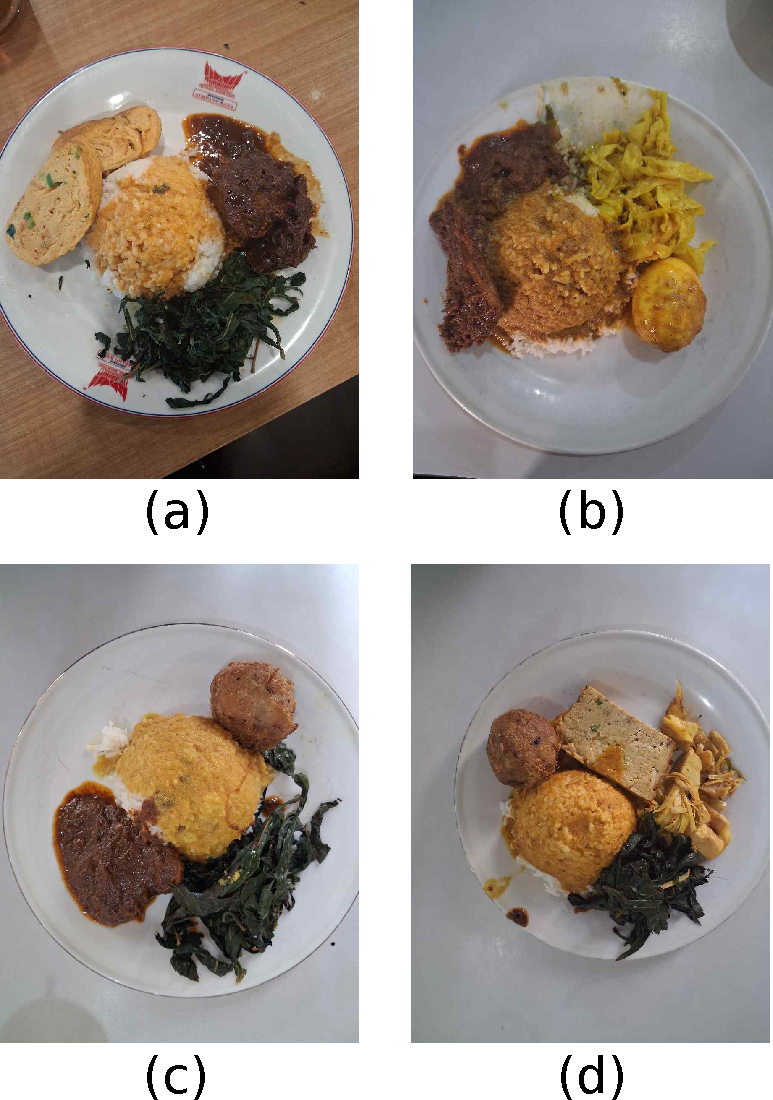
\includegraphics[width=0.55\textwidth]{figures/contoh_dataset.pdf}
		\caption{Contoh citra hasil pengumpulan data secara langsung}
    \label{fig:contoh-dataset}
\end{figure}

\subsubsection{Anotasi Data}

Citra yang telah lolos tahap seleksi dianotasi untuk menghasilkan \textit{ground truth} yang diperlukan dalam pelatihan, validasi, dan pengujian YOLO11-seg. Anotasi dilakukan pada setiap instans objek makanan yang termasuk dalam kelas penelitian menggunakan CVAT.

Anotasi dibuat dalam bentuk poligon yang mengikuti batas objek yang terlihat pada citra. Setiap poligon diberikan label kelas sehingga memuat informasi mengenai jenis dan area objek. Apabila satu citra mengandung lebih dari satu instans dari kelas yang sama, setiap instans dianotasi secara terpisah agar model dapat mempelajari dan menghasilkan \textit{segmentation mask} untuk setiap instans secara individual.

Kelas yang digunakan dalam proses anotasi terdiri atas nasi, rendang, ayam goreng, perkedel, sayur nangka, daun singkong, telur dadar, telur kari, dan sambal. Objek makanan di luar sembilan kelas tersebut tidak diberikan anotasi dan diperlakukan sebagai bagian dari latar belakang.

Pada objek yang mengalami oklusi, poligon mengikuti batas bagian objek yang masih terlihat tanpa memperkirakan area yang tertutup oleh objek lain. Ketentuan ini digunakan agar anotasi tetap didasarkan pada informasi visual yang tersedia pada citra.

Anotasi yang telah dibuat diperiksa kembali untuk memastikan kesesuaian label kelas, ketepatan poligon terhadap batas objek, dan pemisahan setiap instans. Hasil anotasi kemudian disimpan dalam format yang sesuai dengan kebutuhan YOLO11-seg dan digunakan pada tahap pembagian dataset.

\subsubsection{Pembagian Dataset}

Dataset yang telah dianotasi selanjutnya dibagi menjadi data pelatihan, validasi, dan pengujian. Pembagian tersebut dilakukan agar proses pelatihan dan evaluasi menggunakan bagian dataset yang berbeda.

Dataset dibagi dengan proporsi 70\% untuk data pelatihan, 15\% untuk data validasi, dan 15\% untuk data pengujian. Jumlah citra pada setiap bagian ditentukan berdasarkan jumlah akhir citra yang telah lolos tahap seleksi dan anotasi. Pembagian dilakukan dengan memperhatikan keterwakilan sembilan kelas penelitian pada setiap bagian dataset.

Data pelatihan digunakan dalam proses pembelajaran dan pembaruan bobot YOLO11-seg. Data validasi digunakan untuk memantau performa model selama pelatihan dan membantu menentukan model terbaik. Data pengujian disimpan secara terpisah dan hanya digunakan untuk mengevaluasi performa model akhir pada citra yang tidak digunakan dalam proses pelatihan.

Pembagian dataset dilakukan sebelum proses augmentasi untuk mencegah citra asli dan hasil augmentasinya tersebar pada bagian dataset yang berbeda. Citra duplikat, citra yang memiliki kemiripan tinggi, dan citra yang berasal dari sumber dasar yang sama ditempatkan pada bagian dataset yang sama untuk mengurangi risiko kebocoran data \cite{tampu2022}. Augmentasi selanjutnya hanya diterapkan pada data pelatihan.

\subsubsection{Augmentasi Data}

Augmentasi diterapkan pada data pelatihan untuk menambah variasi data yang diterima model selama proses pembelajaran. Penerapan augmentasi bertujuan membantu model mempelajari variasi tampilan objek dan mengurangi kecenderungan model menghafal karakteristik citra tertentu \cite{yang2022}.

Augmentasi dilakukan secara dinamis melalui \textit{pipeline} pelatihan YOLO11-seg. Dengan mekanisme ini, transformasi dapat diberikan ketika data pelatihan dimuat tanpa harus menghasilkan salinan citra baru secara permanen. Transformasi pada citra juga diterapkan pada anotasi sehingga posisi \textit{segmentation mask} tetap sesuai dengan objek setelah augmentasi.

Jenis transformasi dipilih dengan mempertimbangkan karakteristik citra dan kondisi penggunaan sistem. Transformasi dapat mencakup perubahan posisi, skala, orientasi, serta karakteristik warna dan pencahayaan selama transformasi tersebut tidak mengubah identitas utama objek atau menghasilkan kondisi yang tidak relevan terhadap penggunaan sistem.

Augmentasi acak tidak diterapkan pada data validasi dan pengujian agar kedua bagian tersebut tetap digunakan sebagai data evaluasi yang merepresentasikan citra aslinya. Konfigurasi augmentasi yang benar-benar digunakan pada proses pelatihan dicatat pada tahap pembuatan sistem.


\subsection{Analisis Sistem}

Tahap analisis sistem dilakukan untuk menentukan kebutuhan yang diperlukan dalam pengembangan sistem \textit{checkout} otomatis Nasi Padang. Analisis mencakup kebutuhan perangkat keras, perangkat lunak, data, dan fungsi yang harus dijalankan oleh sistem.

Perangkat keras yang diperlukan meliputi:
\begin{enumerate}
    \item kamera untuk memperoleh citra piring dari posisi tetap di atas area pengambilan citra;
    \item perangkat komputasi untuk melakukan anotasi data, pelatihan, validasi, pengujian, dan inferensi YOLO11-seg;
    \item media penyimpanan untuk menyimpan citra, anotasi, bobot model, serta hasil pengujian; dan
    \item area pengambilan citra yang memungkinkan posisi kamera dipertahankan tetap dengan kondisi pencahayaan yang relatif konsisten.
\end{enumerate}

Perangkat lunak yang diperlukan meliputi:
\begin{enumerate}
    \item Python sebagai bahasa pemrograman utama untuk pengolahan data, pelatihan model, dan pengembangan program;
    \item Ultralytics sebagai \textit{framework} yang digunakan untuk pelatihan, validasi, pengujian, dan inferensi YOLO11-seg;
    \item CVAT sebagai perangkat anotasi kelas dan poligon untuk setiap instans objek makanan; dan
    \item pustaka pendukung yang diperlukan untuk pengolahan citra, pengelolaan dataset, serta implementasi program kalkulasi harga.
\end{enumerate}

Data utama yang dibutuhkan berupa citra Nasi Padang beserta anotasi poligon dan label kelas untuk setiap instans. Sistem juga memerlukan tabel harga tetap yang memuat pasangan antara kelas makanan dan harga satuan.

Secara fungsional, sistem harus mampu menerima citra dari kamera, menghasilkan prediksi kelas dan \textit{segmentation mask} untuk setiap instans, menghitung jumlah instans berdasarkan kelas, mencocokkan hasil tersebut dengan tabel harga, serta menghitung subtotal dan total harga. Spesifikasi perangkat dan versi perangkat lunak yang benar-benar digunakan dicatat pada tahap pembuatan sistem.

\subsection{Perancangan Sistem}

Tahap perancangan sistem bertujuan menggambarkan alur kerja sistem \textit{checkout} otomatis Nasi Padang mulai dari pelatihan model hingga penggunaan model pada proses \textit{checkout}. Perancangan dibagi menjadi dua bagian, yaitu rancangan pelatihan model YOLO11-seg dan rancangan proses \textit{checkout}.

Rancangan pelatihan model menjelaskan alur penggunaan dataset yang telah dianotasi dan dibagi menjadi data pelatihan, validasi, dan pengujian. Data pelatihan digunakan untuk melatih YOLO11-seg melalui proses prediksi, perhitungan \textit{loss}, dan pembaruan bobot model. Performa model dipantau menggunakan data validasi hingga diperoleh model akhir yang digunakan dalam proses pengujian dan inferensi.

Rancangan proses \textit{checkout} menjelaskan alur pengolahan citra piring yang diperoleh dari kamera. Model YOLO11-seg menghasilkan prediksi kelas dan \textit{segmentation mask} untuk setiap instans objek makanan. Setiap instans kemudian dihitung berdasarkan kelasnya dan dicocokkan dengan tabel harga tetap untuk memperoleh subtotal setiap kelas serta total harga keseluruhan.

Rancangan pelatihan model dan proses \textit{checkout} dijelaskan lebih lanjut pada subbagian berikut.

\subsubsection{Rancangan Pelatihan Model}

Pelatihan dilakukan menggunakan YOLO11-seg dengan bobot pralatih sebagai titik awal. Bobot tersebut selanjutnya disesuaikan terhadap sembilan kelas makanan pada dataset penelitian sehingga proses pelatihan tidak dimulai dari bobot acak.

Data pelatihan diberikan kepada model dalam bentuk citra beserta \textit{ground truth} yang memuat label kelas dan poligon segmentasi setiap instans. Pada saat data dimuat, citra disesuaikan dengan ukuran masukan model dan dapat menerima augmentasi sesuai konfigurasi pelatihan.

Selama pelatihan, model menghasilkan prediksi yang dibandingkan dengan \textit{ground truth} untuk memperoleh nilai \textit{loss}. Nilai tersebut digunakan dalam proses \textit{backpropagation} dan pembaruan bobot. Proses ini dilakukan berulang selama sejumlah \textit{epoch} yang ditetapkan pada tahap implementasi.

Data validasi digunakan selama pelatihan untuk memantau perkembangan performa model tanpa digunakan untuk memperbarui bobot. Hasil validasi digunakan sebagai dasar pemilihan bobot model yang selanjutnya digunakan pada evaluasi akhir.

Model terpilih kemudian dievaluasi menggunakan data pengujian yang tidak digunakan untuk pembaruan maupun pemilihan bobot. Evaluasi dilakukan terhadap kemampuan model dalam mendeteksi, mengklasifikasikan, membentuk \textit{segmentation mask}, serta menghasilkan jumlah instans yang sesuai dengan \textit{ground truth}. Varian YOLO11-seg, ukuran masukan, jumlah \textit{epoch}, \textit{batch size}, dan konfigurasi pelatihan lainnya dicatat sesuai implementasi yang benar-benar digunakan.

\subsubsection{Rancangan Proses Checkout}

Proses \textit{checkout} dimulai ketika piring yang berisi makanan ditempatkan pada area pengambilan citra. Kamera yang berada pada posisi tetap di atas area tersebut memperoleh citra piring dalam kondisi pencahayaan yang relatif terkontrol. Citra kemudian diberikan sebagai masukan kepada model YOLO11-seg yang telah melalui proses pelatihan.

Pada tahap inferensi, YOLO11-seg memproses citra dan menghasilkan prediksi untuk setiap instans objek makanan. Setiap prediksi memuat lokasi objek, nilai kepercayaan, label kelas, dan \textit{segmentation mask}. Prediksi dengan nilai kepercayaan yang memenuhi batas yang ditentukan dipertahankan sebagai hasil pengenalan.

Label kelas digunakan untuk menentukan jenis objek makanan, sedangkan \textit{segmentation mask} digunakan untuk memisahkan setiap instans yang terdapat pada piring. Setiap hasil prediksi yang dipertahankan diperlakukan sebagai satu instans. Apabila terdapat lebih dari satu instans dari kelas yang sama, seluruh instans tersebut dihitung dan dikelompokkan berdasarkan kelasnya.

Hasil penghitungan kemudian diteruskan ke program kalkulasi harga. Program menggunakan tabel harga tetap yang memuat pasangan antara kelas makanan dan harga setiap instans. Subtotal setiap kelas dihitung dengan mengalikan jumlah instans yang dikenali dengan harga pada kelas tersebut. Seluruh subtotal selanjutnya dijumlahkan untuk memperoleh total harga.

Informasi yang dihasilkan pada proses \textit{checkout} terdiri atas kelas makanan yang dikenali, jumlah instans pada setiap kelas, harga setiap instans, subtotal setiap kelas, dan total harga keseluruhan. \textit{Segmentation mask} tidak digunakan untuk memperkirakan berat, volume, luas porsi, maupun kandungan gizi makanan.

Proses tersebut menghasilkan mekanisme \textit{checkout} otomatis yang menghubungkan hasil pengenalan YOLO11-seg dengan program kalkulasi harga. Sistem dirancang sebagai \textit{proof-of-concept} dan tidak mencakup proses pembayaran elektronik maupun pencetakan bukti pembayaran.


